\documentclass[border=3pt]{standalone}
% Preâmbulo compartilhado pelos diagramas TikZ da aula 5 de IHC (Processos de Design)
\usepackage[T1]{fontenc}
\usepackage[utf8]{inputenc}
\usepackage{lmodern}
\usepackage{amsmath}
\usepackage{xcolor}
\usepackage{tikz}
\usetikzlibrary{arrows.meta,angles,quotes,decorations.pathmorphing,calc,
                positioning,shapes.geometric,shapes.misc,backgrounds,fit,
                math}

% Paleta (mesma dos SVGs originais)
% Paleta da disciplina de IHC: acento roxo (#755099), da capa do livro.
% (o nome "dblue" é mantido para não alterar todos os diagramas)
\definecolor{dblue}{HTML}{755099}
\definecolor{dorange}{HTML}{B3541E}
\definecolor{dgreen}{HTML}{4A7C59}
\definecolor{dred}{HTML}{9C4B4B}
\definecolor{dcream}{HTML}{F4F1EA}
\definecolor{dshade}{HTML}{DDD7C9}

% Função gaussiana (não normalizada por padrão de escala visual)
\pgfmathdeclarefunction{gauss}{3}{%
  \pgfmathparse{1/(#3*sqrt(2*pi))*exp(-((#1-#2)^2)/(2*#3^2))}%
}

% Estilos comuns (prefixo d... para não colidir com chaves internas do pgf)
\tikzset{
  >={Stealth[length=2mm]},
  dguide/.style={gray!55, dashed, line width=0.4pt},
  daxis/.style={gray!60, line width=0.7pt, ->},
  dbody/.style={fill=black!3, draw=black!80, line width=1pt},
  dacc/.style={draw=dblue, line width=1pt},
  dlbl/.style={black!55, font=\small},
  dsub/.style={black!45, font=\footnotesize},
  dstate/.style={circle, draw=black!80, fill=dcream, line width=1pt,
                 minimum size=17mm, font=\large, inner sep=1pt},
  dobs/.style={circle, draw=black!80, fill=dshade, line width=1pt,
               minimum size=14mm, font=\large, inner sep=1pt},
  dbox/.style={rounded corners=2pt, draw=black!80, fill=dcream, line width=1pt,
               align=center, inner sep=6pt},
  dop/.style={circle, draw=black!80, fill=white, line width=1pt,
              minimum size=6mm, inner sep=0pt, font=\small},
  dtrans/.style={->, dblue, line width=1pt},
  dmeas/.style={->, dorange, line width=1pt},
  dcurve/.style={line width=1pt, dblue},
  dcurveb/.style={line width=1.4pt, dorange},
}

\begin{document}
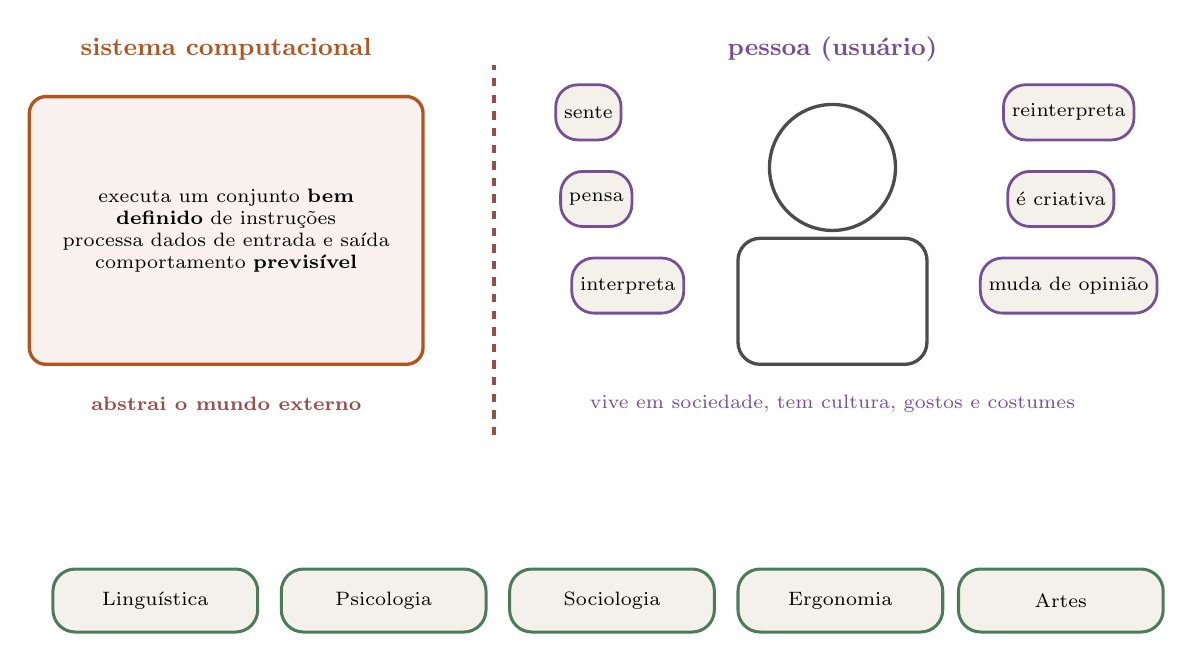
\begin{tikzpicture}[x=1cm,y=1cm,
   chip/.style={dbox, rounded corners=8pt, minimum width=2.6cm, minimum height=0.8cm, font=\scriptsize, draw=dgreen, line width=1.1pt}]

  % sistema
  \node[font=\small\bfseries, dorange] at (2.5,5.4) {sistema computacional};
  \draw[dorange, line width=1.2pt, rounded corners=6pt, fill=dorange!8] (0,1.4) rectangle (5,4.8);
  \node[font=\scriptsize, align=center, text width=4.2cm] at (2.5,3.1) {executa um conjunto \textbf{bem definido} de instruções\\ processa dados de entrada e saída\\ comportamento \textbf{previsível}};

  % pessoa
  \node[font=\small\bfseries, dblue] at (10.2,5.4) {pessoa (usuário)};
  \draw[black!70, line width=1.2pt, fill=white] (10.2,3.9) circle (0.8);
  \draw[black!70, line width=1.2pt, fill=white, rounded corners=8pt] (9.0,1.4) rectangle (11.4,3.0);
  \foreach \x/\y/\t in {7.1/4.6/sente, 7.2/3.5/pensa, 7.6/2.4/interpreta, 13.2/4.6/reinterpreta, 13.1/3.5/é criativa, 13.2/2.4/muda de opinião} {
    \node[dbox, rounded corners=8pt, draw=dblue, minimum height=0.7cm, font=\scriptsize, inner sep=3pt] at (\x,\y) {\t};
  }
  \node[font=\scriptsize, dblue] at (10.2,0.9) {vive em sociedade, tem cultura, gostos e costumes};

  \draw[dred, line width=1.5pt, dashed] (5.9,0.5) -- (5.9,5.2);
  \node[dred, font=\scriptsize\bfseries] at (2.5,0.9) {abstrai o mundo externo};

  % disciplinas
  \foreach \x/\t in {1.6/Linguística, 4.5/Psicologia, 7.4/Sociologia, 10.3/Ergonomia, 13.1/Artes} { \node[chip] at (\x,-1.6) {\t}; }

\end{tikzpicture}
\end{document}
